\chapter{Data Fragmentation}
In a distributed database system, two major questions are:
\begin{itemize}
    \item How the entire set of data items in the database can be split into subsets \(\rightarrow\) \textbf{ data fragmentation (sharding / partitioning)}
    \item How the subsets can be distributed among the database servers in the network \(\rightarrow\) \textbf{data allocation}
\end{itemize}

\section{Properties and Types of Fragmentation}
The query behavior of users plays an important role for the quality of fragmentation and allocation, like the:
\begin{itemize}
    \item Type of access
    \item Access patterns
    \item Affinity of records
    \item Frequency of accesses 
    \item Accesses duration
\end{itemize}
Once a good fragmentation and allocation have been established, a distributed database can take \textbf{advantage} of:
\begin{itemize}
    \item Data locality
    \item Minimization of communication costs
    \item Improved efficiency of data management
    \item Load balancing 
\end{itemize}
However on average a fragmented database system has to live with several \textbf{disadvantages}:
\begin{itemize}
    \item Queries that involve subqueries over different fragments are costly because the global query has to be split into subqueries
    \item Distributed transactions are extremely difficult to manage
\end{itemize}
Several criteria are important when designing a distributed database with fragmented data sets. The most important is that a given data fragmentation must be correct, in the sense that the original data must be \textit{entirely reconstructed}. When the data set is recombined from the fragments, the following two \textbf{correctness properties} are required:
\begin{itemize}
    \item \textbf{Completeness:} none of the original data records is lost during fragmentation and hence no data is missing in the reconstructed data set
    \item \textbf{Soundness:} no additional data are introduced in the reconstructed data set
\end{itemize}

\section{Data Allocation}
For fragmented data a major problem is how to \textit{distribute the fragments} over the database servers. A \textbf{data allocation mechanism} has to decide which fragment should be stored on which server, thus \textbf{load balancing} has to be taken into account. There are several forms of data allocation:
\begin{itemize}
    \item \textbf{Range-based allocation} relies on range-based fragmentation. When a range-based fragmentation is obtained the identified ranges have to be assigned to the available servers
    \item \textbf{Hash-based allocation} uses a hash function on the input fragments to determine which server each fragment is assigned to. With hash-based allocation the distribution of the records among the servers is usually more balanced because the hash function distributes its input values well over its entire output hash values
    \item \textbf{Cost-based allocation} describes the data allocation task as an optimization problem
\end{itemize}

\subsection{Consistent Hashing}
Consistent hashing is an hash-based allocation schema which provides a better and more flexible distribution of the records among a set of servers.
\begin{itemize}
    \item A hash function is computed on each input fragment
    \item The hash values are now seen as a ring that wraps around: when we have reached the highest hash value we start again from 0
    \item A hash value is computed not only for each fragment but also for each database server
\end{itemize}
By computing a hash value for a database server, \textbf{each server} has a \textit{fixed position on the ring}; the advantage of these hash values is that they presumably distribute the servers uniformly on the ring.
\newpage
\begin{tcolorbox}
A widely used allocation policy is then to store data on the next server on the ring when looking in clockwise direction.
\end{tcolorbox}
\begin{figure}[!h]
        \centering
        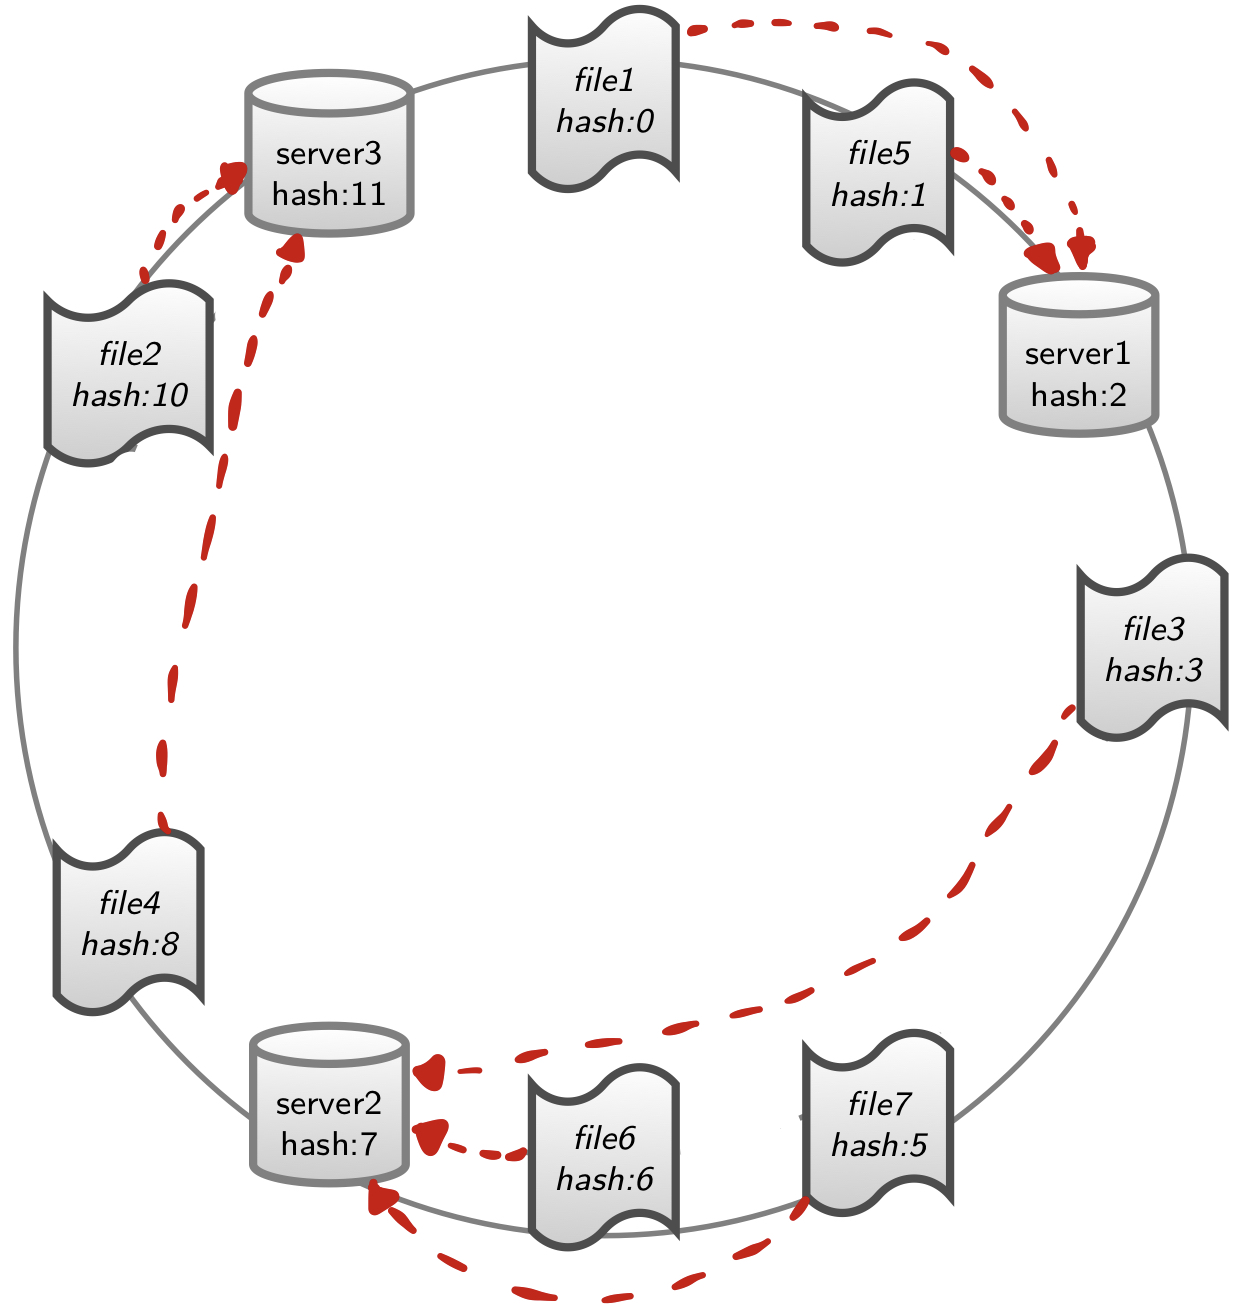
\includegraphics[width=0.4\linewidth]{images/AdvancedDataManagment/data_fragmentation/data_allocation.jpeg}
        \caption{Data allocation with consistent hashing}
    \end{figure}
A major advantage of consistent hashing is its \textit{flexible support} of \textbf{additions} or \textbf{removals} of servers.
\begin{itemize}
    \item Whenever a server \textbf{leaves} the ring: all the data that it stores have to be moved to the next server in clockwise direction
    \begin{figure}[!h]
        \centering
        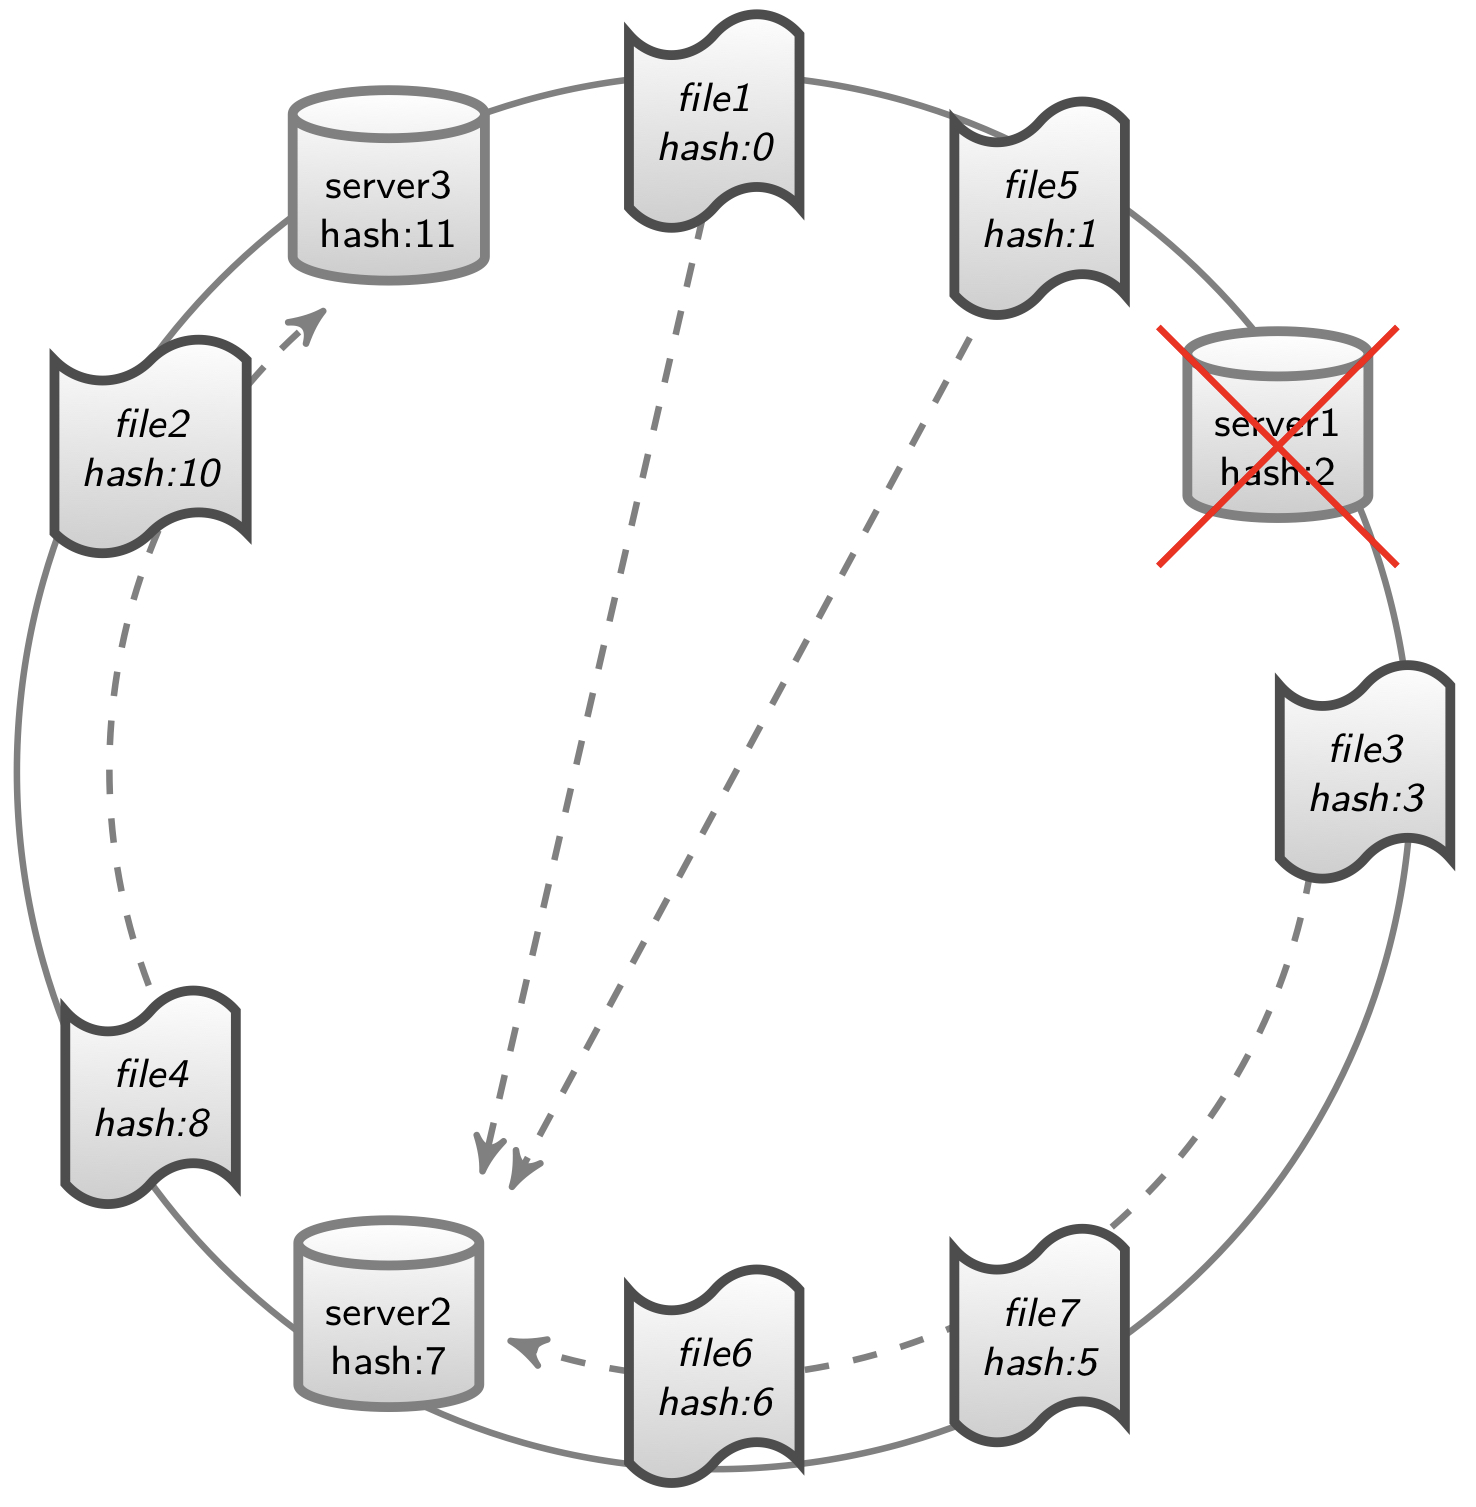
\includegraphics[width=0.4\linewidth]{images/AdvancedDataManagment/data_fragmentation/server_removal.jpeg}
        \caption{Server removal with consistent hashing}
    \end{figure}
    \newpage
    \item Whenever a server \textbf{joins} the ring: the data with a hash value less than the hash value of the new server have to be moved to the new server
    \begin{figure}[!h]
        \centering
        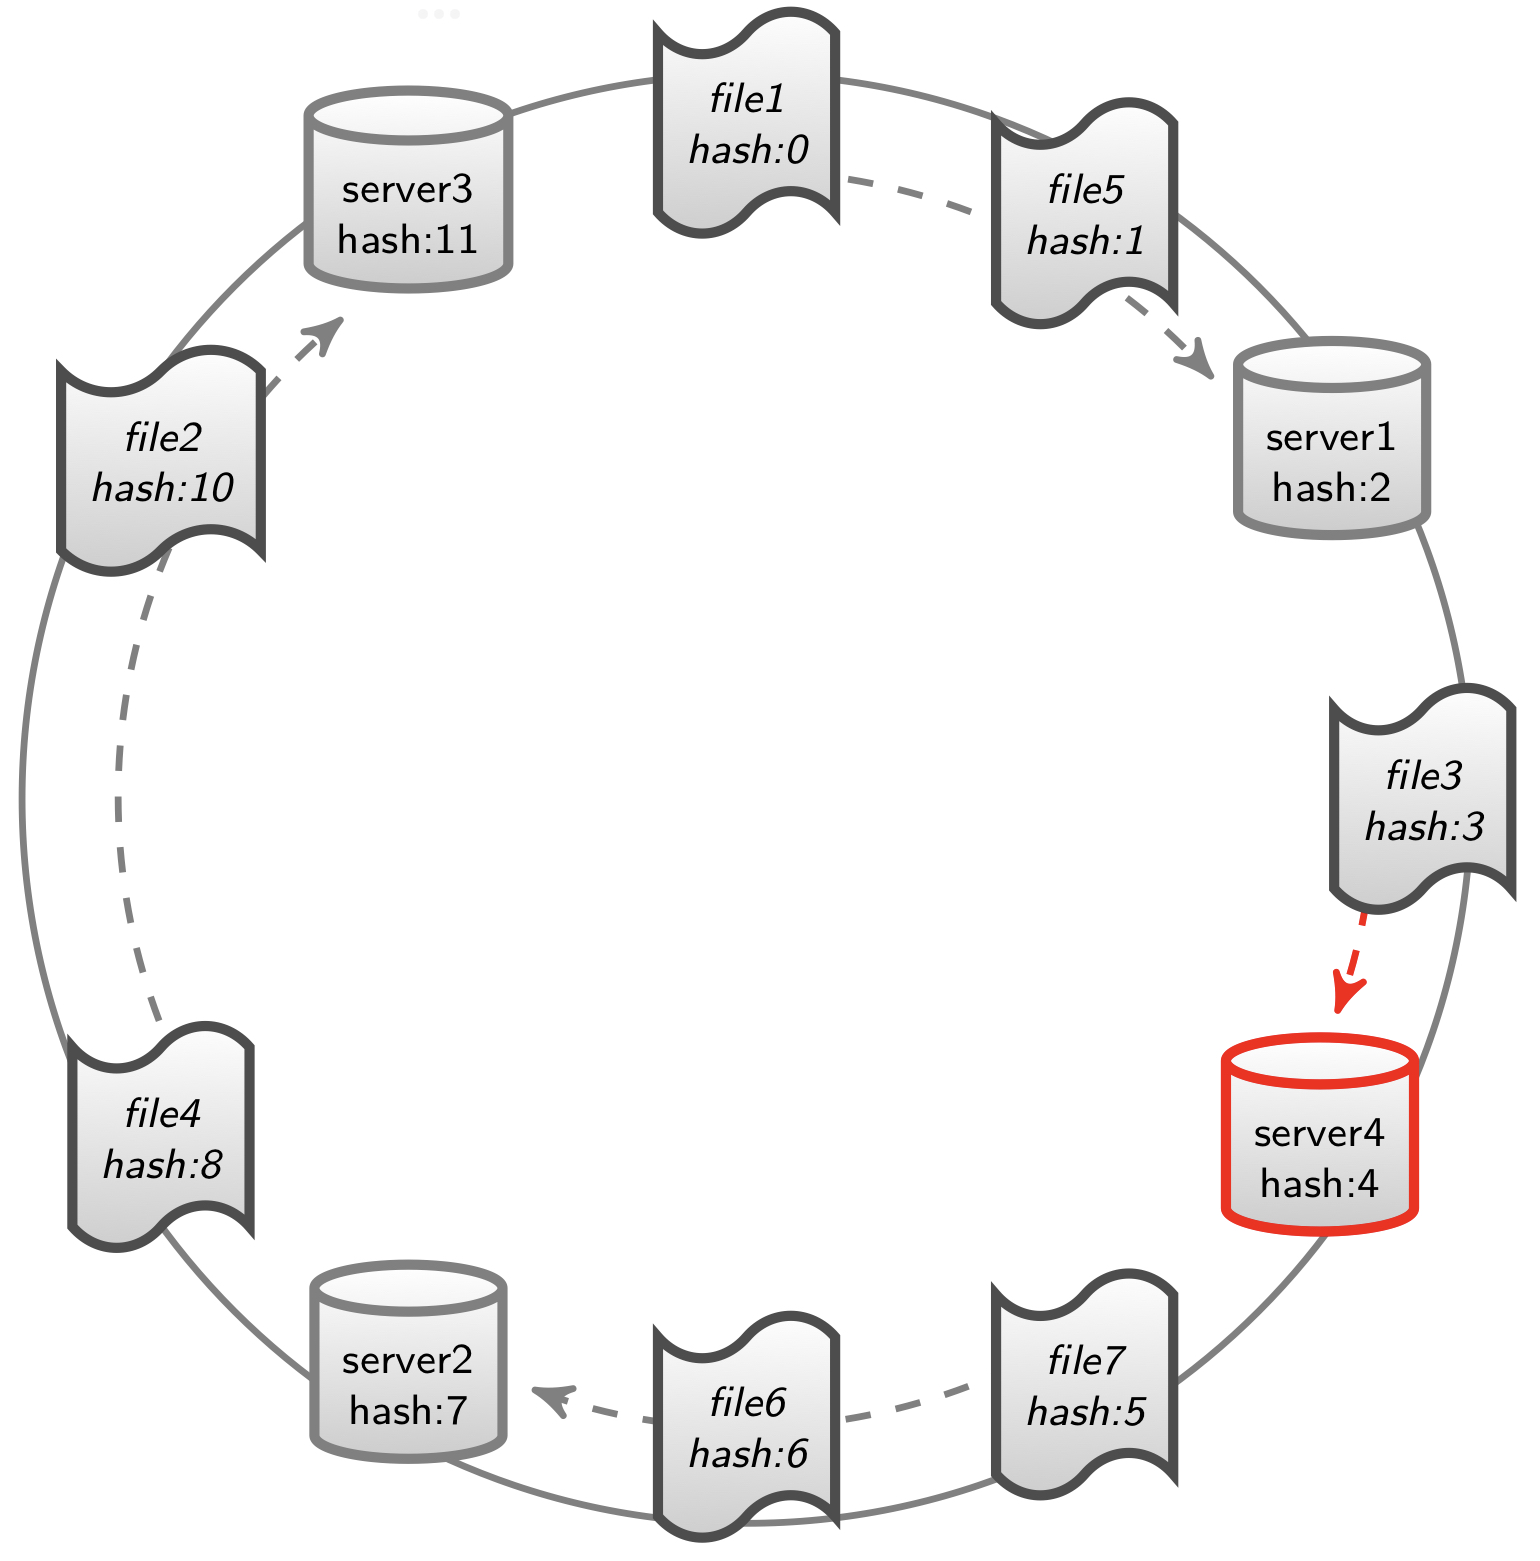
\includegraphics[width=0.4\linewidth]{images/AdvancedDataManagment/data_fragmentation/server_addition.jpeg}
        \caption{Server addition with consistent hashing}
    \end{figure}
\end{itemize}
An important tool to make consistent hashing \textit{more flexible} is to have not only one location on the ring for each physical server but instead to have \textit{multiple locations}: these locations are then called \textbf{virtual servers}. Virtual servers improve consistent hashing in the following cases:
\begin{itemize}
    \item The virtual servers (of each physical server) are spread along the ring in an arbitrary way. So, all servers have a better spread on the ring which leads to a better data distribution
    \item Heterogeneous servers are supported. So a server with less capacity can be represented by less virtual servers than a server with more capacity
    \item New servers can be gradually added to the ring: instead of shifting its entire data load onto a new server at once, virtual servers for the new server can be added one at a time. In this way the new server has tie to start up slowly and take in its full load step by step until its full capacity is reached.
\end{itemize}
\begin{figure}[!h]
        \centering
        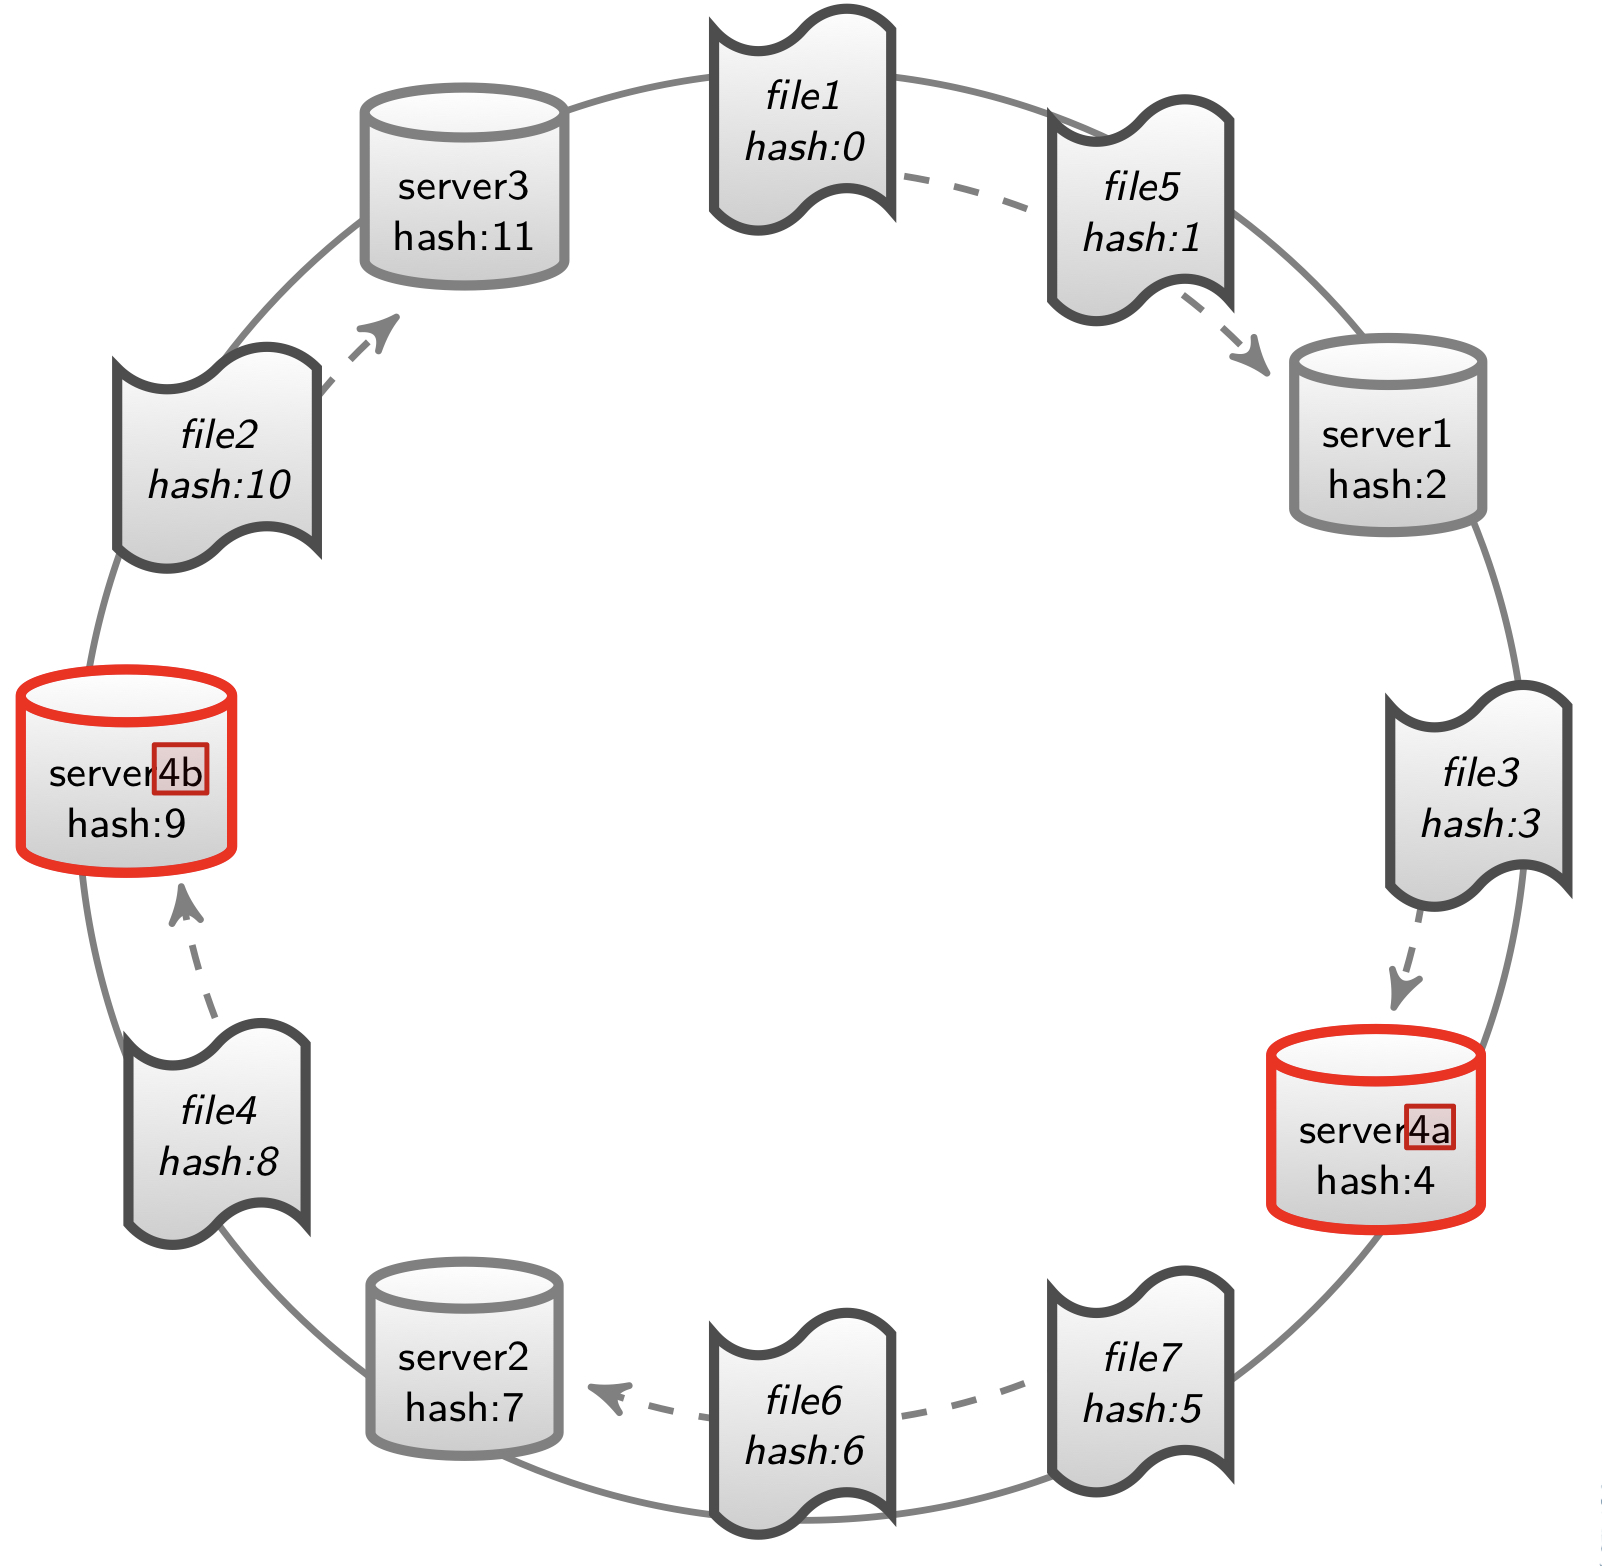
\includegraphics[width=0.4\linewidth]{images/AdvancedDataManagment/data_fragmentation/virtual_servers.jpeg}
        \caption{Virtual server with consistent hashing}
    \end{figure}